\documentclass[11pt]{article}

\usepackage[margin=1in]{geometry}
\usepackage{amsmath, amssymb, amsthm}
\usepackage{enumitem}
\usepackage{tikz}
\usetikzlibrary{circuits.logic.US, positioning}

\pagestyle{empty}

\begin{document}

\begin{center}
  {\Large\bfseries Weekly Assignment: Arguments \& Circuits\\[2pt]
   (Epp~2.3 \& 2.4)}
\end{center}

\bigskip

\noindent
Complete each of the following problems.  Show all work and justify your answers.

\bigskip

%% ─────────────────────────────────────────────
\noindent\textbf{Problem 1} (Epp 2.3 \#9). \;
Use a truth table to determine whether the following argument
form is valid.  Indicate which columns represent the premises
and which represent the conclusion, and include a sentence
explaining how the truth table supports your answer.
\[
  \begin{array}{l}
    p \lor q \to \lnot r \\
    p \lor \lnot q \\
    \lnot q \to p \\
    \hline
    \therefore\; \lnot r
  \end{array}
\]

\bigskip

%% ─────────────────────────────────────────────
\noindent\textbf{Problem 2} (Epp 2.3 \#28). \;
Determine whether the following argument is valid or invalid.
Use symbols to write the logical form of the argument.
If the argument is valid, identify the rule of inference
that guarantees its validity.  Otherwise, state whether the
converse or inverse error is made.

\begin{quote}
  If there are as many rational numbers as there are irrational
  numbers, then the set of all irrational numbers is infinite.\\
  The set of all irrational numbers is infinite.\\
  $\therefore$ There are as many rational numbers as there are
  irrational numbers.
\end{quote}

\bigskip

%% ─────────────────────────────────────────────
\noindent\textbf{Problem 3} (Epp 2.3 \#30). \;
Determine whether the following argument is valid or invalid.
Use symbols to write the logical form of the argument.
If the argument is valid, identify the rule of inference
that guarantees its validity.  Otherwise, state whether the
converse or inverse error is made.

\begin{quote}
  If this computer program is correct, then it produces the
  correct output when run with the test data my teacher gave me.\\
  This computer program produces the correct output when run with
  the test data my teacher gave me.\\
  $\therefore$ This computer program is correct.
\end{quote}

\bigskip

%% ─────────────────────────────────────────────
\noindent\textbf{Problem 4} (Epp 2.3 \#44). \;
Use the valid argument forms listed in Table~2.3.1 to deduce
the conclusion from the premises, giving a reason for each step
as in Example~2.3.8.  Assume all variables are statement
variables.

\[
  \begin{array}{rll}
    \text{a.} & p \to q            \\
    \text{b.} & r \lor s            \\
    \text{c.} & \lnot s \to \lnot t \\
    \text{d.} & \lnot q \lor s      \\
    \text{e.} & \lnot s             \\
    \text{f.} & \lnot p \land r \to u \\
    \text{g.} & w \lor t            \\
    \hline
    & \therefore\; u \land w
  \end{array}
\]

\bigskip

%% ─────────────────────────────────────────────
\noindent\textbf{Problem 5} (Epp 2.4 \#2). \;
Give the output signal for the following circuit if the input
signals are $P = 1$ and $Q = 0$.

\begin{center}
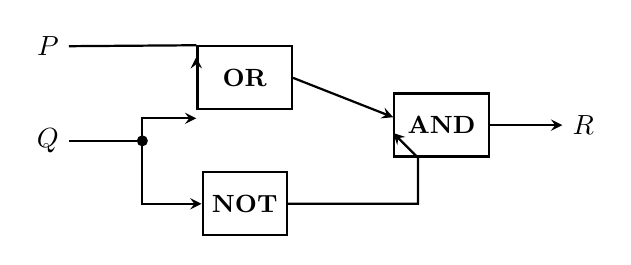
\begin{tikzpicture}[
    gate/.style={draw, minimum width=1.2cm, minimum height=0.8cm,
                 font=\small\bfseries},
    notgate/.style={gate, minimum width=0.9cm},
    thick,
    >=stealth
  ]
  % Input lines
  \node (P) at (0,1) {$P$};
  \node (Q) at (0,-0.2) {$Q$};

  % OR gate
  \node[gate] (or) at (2.5,0.6) {OR};

  % NOT gate
  \node[notgate] (not) at (2.5,-1) {NOT};

  % AND gate
  \node[gate] (and) at (5,0) {AND};

  % Output
  \node (R) at (6.8,0) {$R$};

  % Wiring
  \draw[->] (P) -- (or.west |- or.north west) ++(0,-0.15);
  \coordinate (Qjunc) at (1.2,-0.2);
  \draw (Q) -- (Qjunc);
  \draw[->] (Qjunc) |- ([yshift=-0.1cm]or.south west);
  \draw[->] (Qjunc) |- (not.west);

  \draw[->] (or.east) -- ([yshift=0.1cm]and.west);
  \draw[->] (not.east) -| ([xshift=-0.3cm]and.south) -- ([yshift=-0.1cm]and.west);

  \draw[->] (and.east) -- (R);

  % Junction dot
  \fill (Qjunc) circle (2pt);
\end{tikzpicture}
\end{center}

\noindent
The circuit has inputs $P$ and~$Q$.  The signal~$Q$ branches: one
copy goes (together with~$P$) into an \textbf{OR}~gate, the other
into a \textbf{NOT}~gate.  The outputs of the OR~gate and the
NOT~gate then feed into an \textbf{AND}~gate, producing the
output~$R$.

\bigskip

%% ─────────────────────────────────────────────
\noindent\textbf{Problem 6} (Epp 2.4 \#19). \;
For the input/output table below, construct
\begin{enumerate}[label=\textbf{(\alph*)}]
  \item a Boolean expression having the given table as its
        truth table, and
  \item a circuit having the given table as its input/output
        table.
\end{enumerate}

\bigskip

\begin{center}
\begin{tabular}{ccc|c}
  $P$ & $Q$ & $R$ & $S$ \\\hline
   1  &  1  &  1  &  0 \\
   1  &  1  &  0  &  1 \\
   1  &  0  &  1  &  0 \\
   1  &  0  &  0  &  1 \\
   0  &  1  &  1  &  0 \\
   0  &  1  &  0  &  1 \\
   0  &  0  &  1  &  0 \\
   0  &  0  &  0  &  0 \\
\end{tabular}
\end{center}

\end{document}
